\documentclass[a4paper,12pt]{article}
\usepackage{amssymb} % needed for math
\usepackage{amsmath} % needed for math
\usepackage[utf8]{inputenc} % this is needed for umlauts
\usepackage[ngerman]{babel} % this is needed for umlauts
\usepackage[T1]{fontenc}    % this is needed for correct output of umlauts in pdf
\usepackage[margin=2.5cm]{geometry} %layout
\usepackage{fancyhdr}  % needed for the footer
\usepackage{lastpage}  % needed for the footer
\usepackage{hyperref}  % links im text
\usepackage{color, colortbl}  % farbige Tabellenzellen
\usepackage{pdfpages}  % Signatureinbingung und includepdf
\usepackage{tabularx}
\usepackage[onehalfspacing]{setspace} % eineinhalbfacher Zeienabstand
\clubpenalty  = 10000 % Schusterjungen verhindern
\widowpenalty = 10000 % Hurenkinder verhindern
\newcommand{\quoteitalic}[1]{\glqq{\textit{#1}}\grqq{}} % quotes

\usepackage{myStyle}

%%%%%%%%%%%%%%%%%%%%%%%%%%%%%%%%%%%%%%%%%%%%%%%%%%%%%%%%%%%%%%%%%%%%%
% Hier eigene Daten einfügen                                        %
%%%%%%%%%%%%%%%%%%%%%%%%%%%%%%%%%%%%%%%%%%%%%%%%%%%%%%%%%%%%%%%%%%%%%
\newcommand{\Jahr}{2012 / 2013}         % Typ: "2011 / 2012" oder "2012"
\newcommand{\Semester}{Wintersemester}  % "Wintersemester" oder "Sommersemester"
\newcommand{\Datum}{\today}             % Wann wurde der Bericht erstellt?
\newcommand{\Ort}{Karlsruhe}
\newcommand{\Vorname}{Max}
\newcommand{\Nachname}{Mustermann}
\newcommand{\Matrikelnummer}{123456}
\newcommand{\Studienfach}{Informatik (BA)}
\newcommand{\Institut}{Institut für Theoretische Informatik}
\newcommand{\TutoriumTitle}{Programmieren Tutorium}
\newcommand{\Email}{info@martin-thoma.de}
%%%%%%%%%%%%%%%%%%%%%%%%%%%%%%%%%%%%%%%%%%%%%%%%%%%%%%%%%%%%%%%%%%%%%
\hypersetup{ 
  pdfauthor   = {\Vorname~\Nachname}, 
  pdfkeywords = {KIT; \Vorname~\Nachname}, 
  pdftitle    = {Abschlussreflexion von~\Vorname~\Nachname~-~\Semester~\Jahr} 
} 
 
\pagestyle{fancy}
\fancyhf{}
\renewcommand{\headrulewidth}{0pt}
\renewcommand{\footrulewidth}{0pt}
\fancyfoot[R]{Seite~\thepage~von \pageref{LastPage}}
 
\definecolor{LightCyan}{rgb}{0.88,1,1}
\definecolor{LightGreen}{rgb}{0.68,1,0.68}
\definecolor{Rosa}{rgb}{1,0.68,0.68}
 
\pagenumbering{arabic}
 
\begin{document}
 \pagenumbering{roman}
 \begin{titlepage}
\thispagestyle{empty}
\ifAFive
    \par\vspace{4cm}
\else
    \par\vspace{10cm}
\fi
\begin{center}
{\Large \textbf{Einführung in die}} \\[2ex]
{\Large \textbf{Geometrie und Topologie}}
\vfill

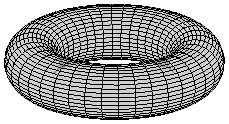
\includegraphics[width=0.9\linewidth]{figures/Torus.pdf}
\vfill
\hrulefill
\end{center}
\ \\[-5ex]
0. Auflage, \today \hfill Martin Thoma
\end{titlepage}

 \setcounter{page}{2}
 \pagenumbering{arabic}

% \title{Semesterbericht über das \Semester \Jahr}
% \author{\Vorname \Nachname}
% \date{\Datum}

\section*{bla}

Lorem ipsum dolor sit amet, consectetur adipiscing elit. Nam auctor consectetur risus, nec condimentum diam fringilla eu. Nullam vel nunc diam. Donec eu justo sed urna consectetur fringilla nec quis purus. Nulla facilisi. Proin ultrices, lacus ut malesuada vehicula, diam eros adipiscing eros, non egestas dolor velit quis purus. Duis semper placerat condimentum. Vestibulum lacinia lobortis nunc, in pretium ligula sagittis sed. In consectetur purus rhoncus odio varius consequat. Praesent semper imperdiet erat id sagittis. Proin elit mi, sagittis eu interdum vitae, tincidunt ut dui.

Nam id est ac augue fermentum varius eget blandit mauris. Donec molestie, lectus et sodales porttitor, augue ipsum volutpat enim, vel pretium erat odio vel magna. Pellentesque sollicitudin orci eget nulla faucibus egestas. Pellentesque aliquet pulvinar sapien, non pretium nulla malesuada vitae. Vestibulum sem augue, fermentum sit amet laoreet ut, laoreet molestie libero. Sed semper, urna sit amet consequat interdum, enim quam eleifend eros, vel luctus neque enim at dui. Vivamus gravida nunc ut sem porttitor bibendum. Sed at neque eu ante mollis ullamcorper. Vestibulum hendrerit massa at tellus porttitor sed lacinia sem eleifend. Etiam turpis magna, imperdiet ut egestas ut, lacinia et dolor. Aenean faucibus, nunc ut faucibus mollis, velit magna ornare sem, a varius erat nulla id lectus. Integer fringilla felis vulputate lacus malesuada non facilisis diam accumsan. Vivamus felis elit, tempus at lacinia et, congue at arcu. Nunc aliquam pretium faucibus. Maecenas dui dui, dapibus quis aliquet ac, aliquet in lectus.


\noindent \Ort, den \Datum\\
\\

\includegraphics[height=10mm]{max-mustermann.pdf}\\
\Vorname~\Nachname
\end{document}
